
\begin{frame}[ctb!]
  \frametitle{Analytical Models}
  \begin{itemize}
    \item Specific Temperature Integral 
    \item Specific Temperature Change 
    \item Lumped Parameter Model and ANL model
    \item Fully Analytic LLNL Model
  \end{itemize}
\end{frame}


\begin{frame}
  \frametitle{Repository Layouts}
  \begin{minipage}{0.3\textwidth}
    \begin{figure}[h!]
      \includegraphics[width=\textwidth]{boreholes.eps}
    \end{figure}
    \begin{figure}[h!]
      \includegraphics[width=\textwidth]{vertical.eps}
    \end{figure}
  \end{minipage}
  \hspace{0.01cm}
  \begin{minipage}{0.3\textwidth}
    \begin{figure}[h!]
      \includegraphics[width=\textwidth]{horizontal.eps}
    \end{figure}
    \begin{figure}[h!]
      \includegraphics[width=\textwidth]{alcoves.eps}
    \end{figure}
  \end{minipage}
  \hspace{0.01cm}\large{$=$}\hspace{0.01cm}
  \begin{minipage}{0.3\textwidth}
    \begin{figure}[b]
      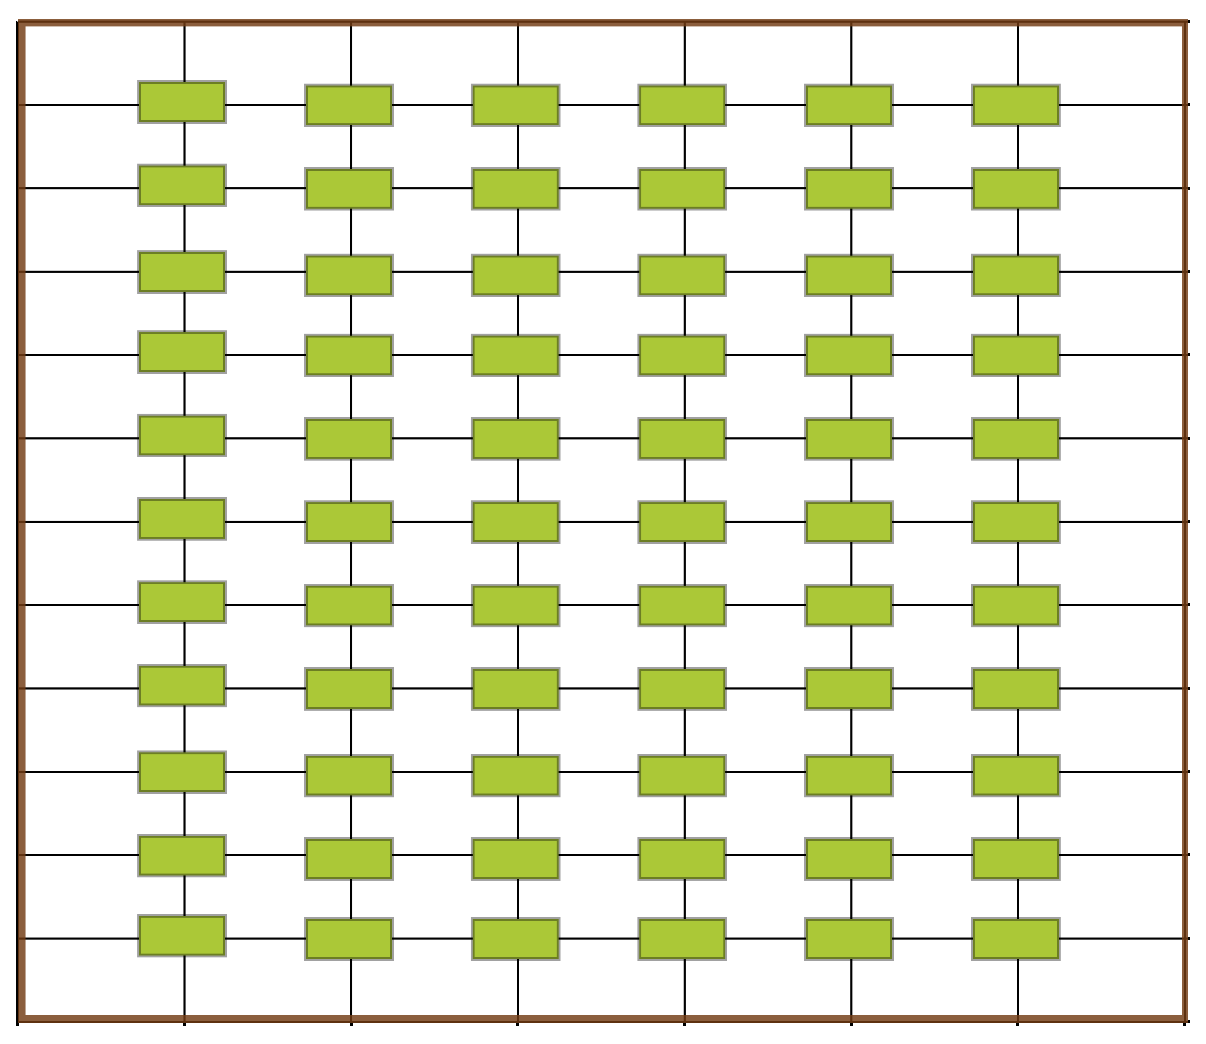
\includegraphics[width=\textwidth]{fullGrid.eps}
    \end{figure}
  \end{minipage}
\end{frame}


\begin{frame}[ctb!]
  \frametitle{Heat Limits In Geology}
  % table?
  Important heat limits in materials of the repository restrict loading designs 
  and capacity.
\end{frame}

% heat based capacity 
\begin{frame}[ctb!]
  \frametitle{Heat Based Capacity}
  % lines, points, infinite lines, footprints.
  \begin{minipage}{0.49\textwidth}
    \begin{figure}[h!]
        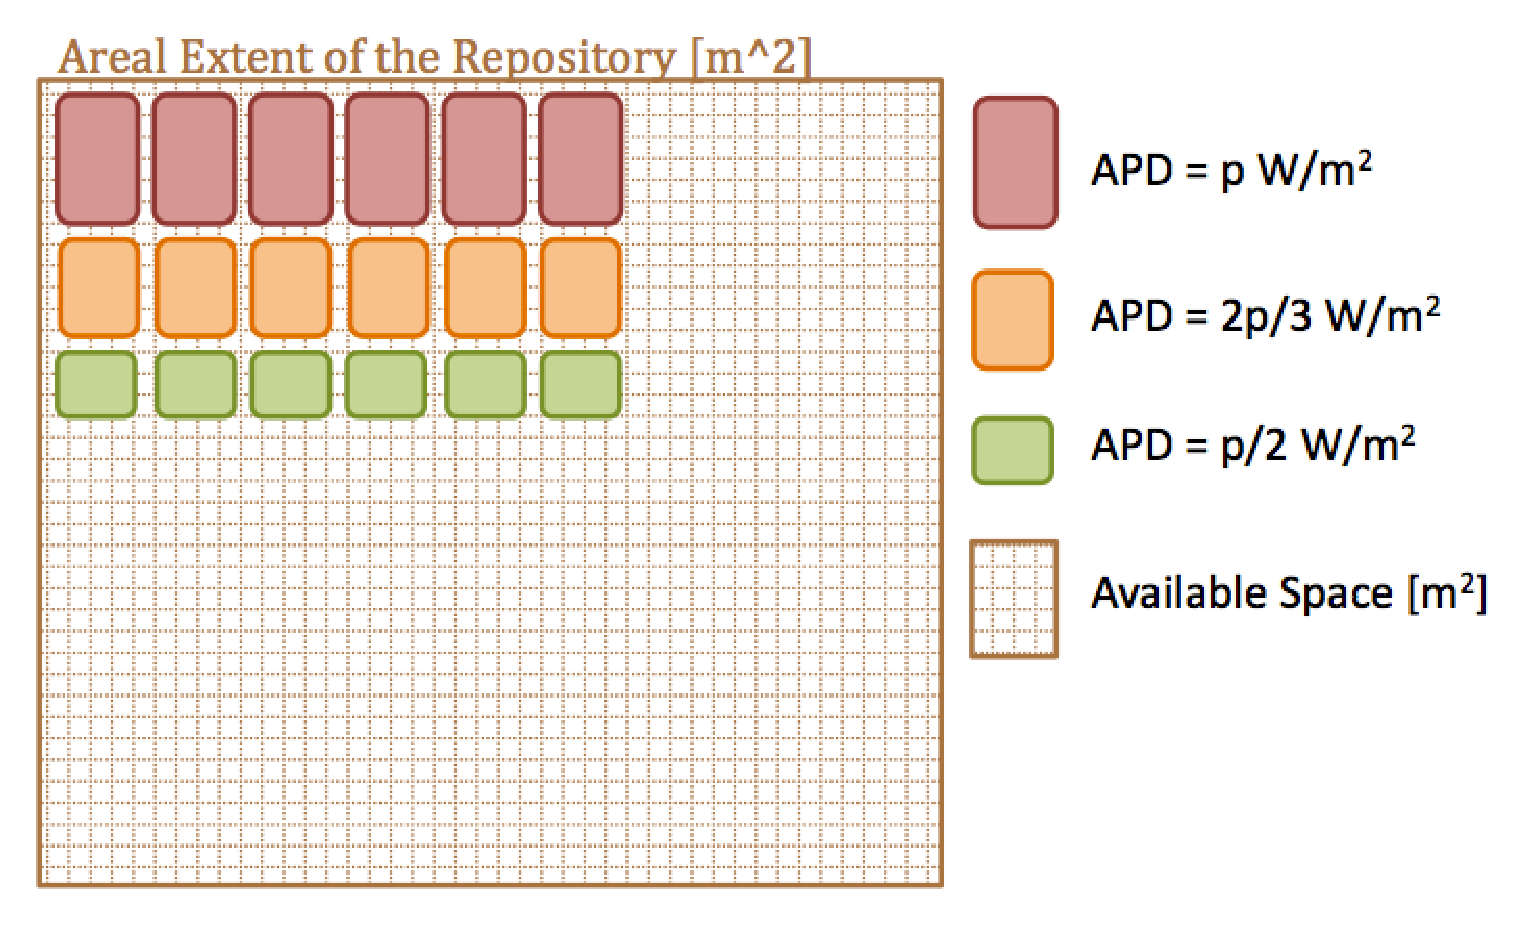
\includegraphics[width=\textheight]{APD.eps}
      \caption{Areal Power Density (APD) can be used to determine appropriate 
      repository loading for arbitrary waste strems.  }
      \label{fig:apd}
  \end{figure}
  \end{minipage}
  \hspace{0.01cm}
  \begin{minipage}{.49\textwidth}
    Loading is subject to the constraints,
    \begin{align}
      P_{tot} &\le P_{max} \\
      APD_i &\le APD_{max}\\
      \label{APD}
      \intertext{where}
      P_{max} &= A\cdot APD_{max} 
      P_{tot} &= \sum_{i=0}^{N}n_i P_i\\ 
      P_{tot} &= \mbox{total power from N packages}\nonumber\\
      P_i &= \mbox{power from package i}\nonumber\\
      n_i &= \mbox{ith waste package}\nonumber\\
      N &= \mbox{number of waste packages}\nonumber\\
      A &= \mbox{areal extent}\nonumber\\ 
      APD_{max} &= \mbox{maximum repository areal power density.}\nonumber
    \end{align}
  \end{minipage}

  
\end{frame}

% heat based capacity 
\begin{frame}[ctb!]
  \frametitle{Impact of Repository Designs}
  % lines, points, infinite lines, footprints.
   \begin{table}[h!]
  \centering
      \footnotesize{
      \begin{tabularx}{\textwidth}{|X|c|c|X|}
          \multicolumn{4}{c}{\textbf{Yucca Mountain Footprint Expansion Calculations}}\\
          \hline
          Author&Max. Capacity&Footprint&Details\\
          &$tonnes$&$km^2$&\\
          \hline
          &&&\\
          OCRWM&$70,000$&$4.65$&``statutory case''\\
          &$97,000$&$6$&``full inventory case''\\
          &$119,000$&$~7$&``additional case''\\
          \hline
          &&&\\
          Yim, M.S.&$75,187$&$4.6$&SRTA code\\
          &$76,493$&$4.6$&STI method\\
          &$95,970$&$4.6$&$63$m drift spacing\\
          &$82,110$&$4.6$&75 yrs. cooling\\
          \hline
          &&&\\
          Nicholson, M.&$103,600$&$4.6$&drift spacing\\
          \hline
          &&&\\
          EPRI&&&\\
          &$63,000$&$6.5$&Base Case CSNF\\
          option 1&$126,000$&$13$&expanded footprint\\
          option 2&$189,000$&$6.5$&multi-level design\\
          option 3&$189,000$&$6.5$&grouped drifts\\
          options 2+3&$252,000$&$6.5$&hybrid\\
          options 1+(2or3) &$378,000$&$13$&hybrid\\
          options 1+2+3 &$567,000$&$13$&hybrid\\
          \hline
        \end{tabularx}
        \caption[Yucca Mountain footprint expansion calculations.]{Various analyses based on heat 
        load limited repository designs have resulted in footprint expansion calculations of the 
        YMR.} 
        \label{tab:footprint}
        }
      \end{table}

\end{frame}




\begin{frame}[ctb!]
  \frametitle{Lumped Parameter Technique}
  % resistor diagram
  \begin{figure}[h!]
    \begin{center}
      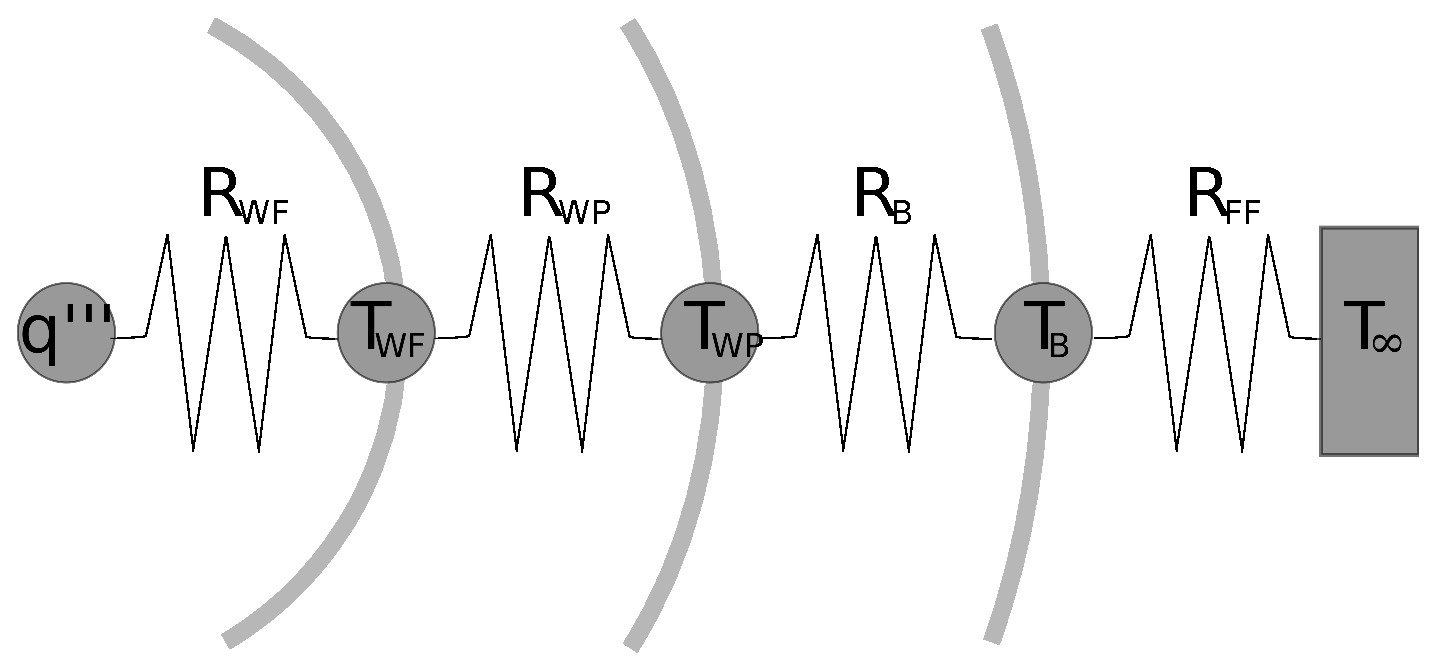
\includegraphics[width=0.9\textwidth]{lumpedParam.eps}
    \end{center}
    \caption{The lumped parameter analogy used for heat transfer can be applied 
    to the one dimensional approximation to the disposal system concept. }
    \label{fig:lumpedParam}
  \end{figure}
  
\end{frame}


% SINDA 

\begin{frame}
  \frametitle{ANL model}
  A model created by the UFD team at Argonne national lab using the 
  SINDA{\textbackslash}G heat transport framework employs a lumped parameter 
  model and an optimization loop to arrive at a minimal drift spacing for a 
  given waste stream in agreement with user input thermal limits. 
  \begin{figure}[h!]
    \begin{center}
      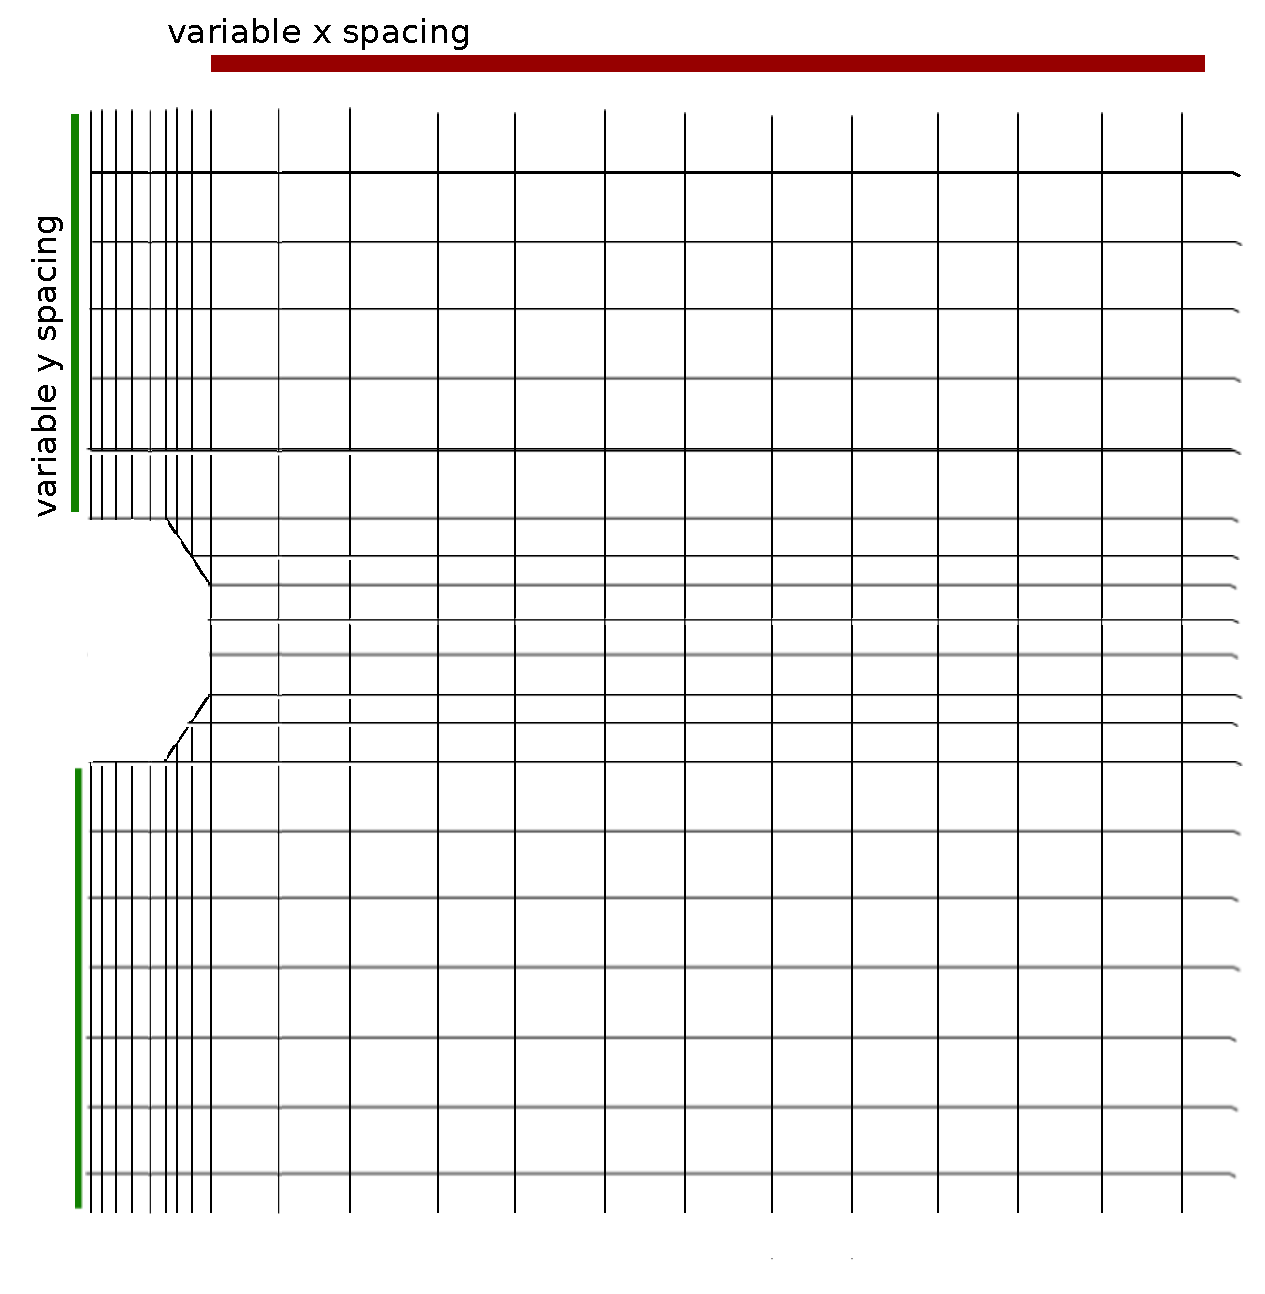
\includegraphics[height=.5\textheight]{../report/litrev/sindageom.eps}
    \end{center}
    \caption{Two adjustable geometric dimensions of the ANL model 
    \cite{bauer_something_2010}.}
    \label{fig:sindageom}
  \end{figure}
\end{frame}

% LLNL

\begin{frame}
  \frametitle{LLNL Model : Geometry}
  \begin{figure}[h!]
    \begin{center}
      \includegraphics[width=0.7\textwidth]{llnlConcept.eps}
    \end{center}
    \caption{Vertical, horizontal, alcove, and borehole emplacement layouts can 
    be represented by a line of point sources and adjacent line sources 
    \cite{greenberg_thermal_2011}.}
    \label{fig:llnl}
  \end{figure}
\end{frame}

\begin{frame}
  \frametitle{LLNL Model : Solution Strategy}
    A MathCAD solution of the transient homogeneous 
    conduction equation,
    
    \begin{align}
      \nabla^2T  = \frac{1}{\alpha}\frac{\partial T}{\partial t}.
      \label{condGl}
    \end{align}
    
    Superimposed point and line source solutions allow for a notion of the repository 
    layout to be modeled in the host rock. The solution of this equation at the 
    boundary of the EBS and the waste package is then treated as a boundary condition 
    for the heterogeneous steady state equation, 
    
    \begin{align}
      \dot{q} &= U A_{out} \left( T_{in} - T_{out} \right)
      \label{condGeneral}
      \intertext{where}
      U&=\frac{1}{\sum_{i}R_i}
      \intertext{which, for the detailed EBS becomes}
      U&=\frac{1}{R_{WF}+R_{WP}+R_{buffer}+\cdots}
    \end{align}
    
    which calculates a resulting temperature gradient through the geometry at each 
    point in time for each layer surface, assuming an infinite line source 
    \cite{hardin_generic_2011}. 
  
\end{frame}



% Loading


\begin{frame}
  \frametitle{Heat Based Drift Loading}

  
\end{frame}

\begin{frame}[ctb!]
  \frametitle{Detailed Techniques}
  % 2d,3d,finite diffs, etc.
   \begin{table}[h!]
    \centering
    \footnotesize{
    \begin{tabular}{|l|c|c|l|}
      \multicolumn{4}{c}{\textbf{Models of Heat Load for Various Geologies}}\\
      \hline
      Source & Nation & Geology & Methodology \\  
      (Who) & (Where) & (What) & (How) \\  
      \hline
      Enresa \cite{von_lensa_red-impact_2008}           & Spain       & Granite       &  CODE\_BRIGHT  \\ 
      NRI   \cite{von_lensa_red-impact_2008}            & Czech Rep.  & Granite       &  Specific Temperature Integral   \\
      ANDRA \cite{andra_granite:_2005}                  & France      & Granite       &  3D Finite Element CGM code   \\
      SKB \cite{ab_long-term_2006}                      & Sweden      & metagranite   &  Forsmark / Laxemar Site \\
                                                        &             &               &  Descriptive Model (SDM)\\
      SCK$\cdot$CEN   \cite{von_lensa_red-impact_2008}  & Belgium     & Clay          &  Specific Temperature Integral   \\ 
      ANDRA \cite{andra_argile:_2005}                   & France      & Argile Clay   &  3D Finite Element CGM code   \\
      NAGRA \cite{johnson_project_2002, johnson_calculations_2002}  & Switzerland  & Opalinus Clay &  3D Finite Element CGM code \\
      GRS \cite{von_lensa_red-impact_2008}              & Germany     & Salt          &  HEATING (3D finite difference)   \\ 
      NCSU(Li)   \cite{li_examining_2007}               & USA         & Yucca Tuff    &  Specific Temperature Integral \\        
      NCSU(Nicholson) \cite{nicholson_thermal_2007}     & USA         & Yucca Tuff    &  SRTA and COSMOL codes\\
      Radel \& Wilson \cite{radel_repository_2007}      & USA         & Yucca Tuff    &  Specific Temperature Change \\ 
      \hline
    \end{tabular}
    \caption[Models for Heat Transport for Various Geologies]{Methods by which to calculate heat 
    load are independent of geology. Maximum heat load constraints, however, vary among host formations. }
    \label{tab:heat}
    }
  \end{table}

  Similar heat transport models can be used for all geologies, but are 
  differentiated by material parameters $(c_p, K, \rho)$ and different 
  thermal constraints.
\end{frame}
